\documentclass{article}
\usepackage{float}
\usepackage{floatrow}
\usepackage[english, serbian c]{babel}
\usepackage[utf8]{inputenc}
\usepackage[T2A]{fontenc}
\usepackage{graphicx}
\usepackage[colorlinks=true, allcolors=blue]{hyperref}

\title{О култури, технологији и глобалним градовима\\
    \small{Семинарски рад у оквиру курса\\Рачунарство и друштво\\Математички факултет Београд}}
\author{Сара Селаковић\\mi17017@alas.matf.bg.ac.rs}

\begin{document}
\maketitle

\begin{abstract}
Технологија је свакодневно све напреднија и очигледан је напредак у различитим областима које знатно утичу на животни стил људи. Велики утицај технологије на друштво огледа се у транспортном и туристичком сектору, у којима се бележи инкрементални раст због значајног пораста броја људи са средњим приходима. Међутим, како примена технолошки настројених решења све више расте, јављају се ризици који се могу одразити на урбану форму, одлуке управљања и очување урођеног идентитета места. У овом раду објашњено је које све ризике са собом доносе глобализација, модернизација и све већа примена технологије у туристичким секторима великих градова.

\end{abstract}

\newpage
\tableofcontents
\newpage

\section{Увод}

Између 20. и 21. века свет је доживео промене великих размера. Међу њима је и појава технологије која је довела до промена у различитим секторима. Што се тиче туризма, број оних који путују у различите дестинације је значајно повећан. Светска туристичка организација (2012) истиче да је до 1950. године годишњи број путника широм света био само 25 милиона, а до 2011. број оних који путују порастао је на 990 милиона \cite{wto}. За то је заслужан напредак у технологији и транспортном сектору, посебно ваздушном саобраћају. Потенцијал туристичке индустрије има директан утицај на градове, који су најчешће циљна дестинација за путовања, а ако то није случај, већина главних саобраћајних чворишта се налази у градовима. Стога је таква популација присиљена да на овај или онај начин ступа у интеракцију са урбаним ткивом.

Схватајући овај потенцијал, локалне самоуправе и градске управе повећавају своја улагања у дигиталне инфраструктуре за подршку новом приливу посетилаца. Такве инвестиције, које се фокусирају на обезбеђивање објеката намењених да привуку посетиоце, нису безазлене јер градови и предузећа разумеју значајне економске користи овог тржишта и његов утицај на локалну економију. Дигитална решења, као што је коришћење мобилних апликација за тражење такси услуга, трансформишу аутомобилску индустрију, посебно у смањењу трошкова паркинга и смањењу саобраћаја. Поред захтева за такси, појавиле су се и мобилне апликације и веб-сајтови који путницима омогућавају да резервишу и закажу своје путовање путем интернета, па стога имају погодност да не морају да чекају у реду, путују до туристичких агенција или чак носе готовину да би извршили плаћања.

\subsection{Млади и путовања}
Како погодности путовања настављају да напредују са новим технологијама, таква практична путовања могу бити популарна и код старије генерације. За њих су пожељне удобност и сигурност, а с друге стране, на одлуке о путовању младих утичу културне атракције које различити градови нуде. Ова демографска група заинтересована је за незаборавне тренутке, што се данас приписује погодностима мобилних уређаја са могућношћу да ухвате и поделе такве тренутке у реалном времену са широм публиком \cite{frommj}. Доста времена проводе на интернету претражујући и упоређујући дестинације које нуде врхунска искуства по што приступачнијим ценама, а заинтересовани су чак и да путују локално све док су садржаји које траже доступни. За њих није важно да ли путују по својој земљи или у иностранству, већ траже доступност локалних искустава попут хране, уметности и природе која су довољна да нахране њихове жеље за путовањем. Овакве трендове младе генерације треба посматрати као могућности великих градова, који би требало да на њих одговоре тако што ће се брендирати на такав начин да би посетиоци пронашли задовољство и узбуђење у њивовим областима. Током брендирања, локалне власти треба да се потруде око дигиталне инфраструктуре јер су оне компатибилније са младима и посебно да максимизирају потенцијал друштвених медија, који су међу млађом популацијом најчешће коришћени начин комуникације. Преко 87\% младе генерације верује друштвеним медијима при инспирацији за путовања, а то значи скоро 46\% успешних резервација, па би градско руководство требало да води рачуна о таквим статистикама \cite{oggA}. Такође, млади су осетљиви на цене, али би били вољни да потроше и преко својих буџетских ограничења ако циљне дестинације нуде јединствене садржаје који се могу поделити преко друштвених медија \cite{starcevic}.

\subsection{Последице технологије у туризму}
Док је економска улога туризма очигледна, улога технологијe може да има негативне последице јер може довести до хомогености урбаног ткива кроз популарне модернистичке идеологије и методе планирања. Модерне градове карактерише окружење које обухвата пет главних индикатора урбаног ткива: варијансу, кохезију, фрагментацију, густину и компактност. Да би се ово постигло, градови, посебно они аутохтони, су погођени јер је већина њихових архитектонских дела демонтирана, рушена, деформисана или подвргнута реновирању. Такве праксе, иако дају жељене резултате, угрожавају посебност и културне аспекте градова, и на крају негативно утичу на њихову атрактивност, посебно у погледу културног туризма. Хомогенизација урбаног ткива угрожава културну разноликост и на тај начин умањује аутентичност и интегритет градова који помажу у њиховој тежњи да буду јединствени и привлачни културним путницима \cite{meyer}. Урбани развој би требало да се заснива на месту које строго поштује, подржава и настоји да промовише културу и традицију заједница које чине пребивалиште градова \cite{unhabitat3}. Тиме се поново ствара применљивост и важност дигиталне технологије јер би она могла да буде кључно средство за убрзавање брендирања старих и културних градова како би се избегла хомогеност и пропадање културе у градовима.

\section{Глобални градови и разноликост}

У протеклих неколико деценија, услед глобализације која је гарантована технолошким напретком, примећени су неки трендови који су пореметили глобалне секторе као што су транспорт и комуникација, уметност и култура, образовање и здравство. Знатно је повећан број путовања, све више преко авио-компанија и бродова за крстарење. Према извештају Међународне асоцијације за ваздушни превоз (2018) \cite{avioni}, број коришћених услуга авио-путовања у 2017. достигао је највиши ниво од 4,1 милијарду, што представља повећање од 7,3\% у односу на број оних који су путовали у 2016. години. Предвиђало се да ће број наставити да расте и достигао је преко 4,6 милијарди људи до краја 2019 \cite{mazarenau}. Што се тиче коришћења бродова за крстарење, подаци Међународне асоцијације крстарења из 2019. године показују да се број путника на крстарењима широм океана стално повећава \cite{kennedy}. На пример, 2015. године било је само 23 милиона таквих путника, али је од 2017. тај број порастао на 26,7 милиона, а до краја 2019. достигао је 30 милиона путника. За разлику од авионског саобраћаја, за оне који се укрцавају на бродове за крстарење се сматра да су жељни нових и егзотичних искустава, посебно у оним удаљеним областима које су углавном доступне путем крузера. Овакви подаци о путовањима само показују значај који путовања представљају за градове и урбане средине.

\subsection{Концепт глобалних градова}
У складу са горе наведеним, градови пружају нову инфраструктуру и објекте који омогућавају бољу интеракцију са тим туристима \cite{postma}. Конкретно, градови су проширили свој низ објеката како би осигурали максималну удобност и искуство путујућих туриста. На пример, сада је могуће имати кухиње и ресторане са различитих удаљених места у истом граду; дакле, туристи имају опције, тако да нема смисла препуштати град другом за такве услуге или искуства. Такође, у данашњем дигиталном добу људи не морају дуго да путују да би отишли у куповину одређеног или јединственог производа у одређеним градовима, као раније када су градови идентификовани са јединственим производима или културама које су искључиво у њима пронађене \cite{zukins}. Са технолошким напретком, сада је могуће имати такве производе у различитим градовима или у различитим продавницама у истом граду у исто време без икаквог компромиса у погледу квалитета или цене. Сматра се да такве стратегије постављају \textit{концепт глобалних градова}.

Очигледно је да овакви трендови ширења искустава у једном граду негативно утичу на културни и урођени идентитет градова. То на крају доводи до хомогених пејзажа што, према урбанистима, води до погоршања културне вредности града \cite{jacobsj}, \cite{alexanderc}, \cite{seamond}. Када се то догоди, граду је тада тешко да створи бренд или имиџ који би пружио јединственост и привлачност, што му отежава повећање способности да привуче ново тржиште културног туризма \cite{hocaoglu}.

\subsection{Превазилажење хомогености у градовима}
Изазов хомогености је премостив ако град одлучи да уклопи технологију у своје урбано ткиво, стварајући на тај начин могућност да задовољи многе културне захтевее за којима путници жуде \cite{allamz1}, \cite{allamz2}. Технологија омогућава поновно успостављање тих изгубљених наслеђа претварајући их у облике који привлаче и односе се на различите демографске групе које чине модерне културне туристе. \textit{Проширена стварност} (\textit{augmented reality}, \cite{ar}) и \textit{виртуелна реалност} (\textit{virtual reality}, \cite{vr}) су међу најпопуларнијим технологијама данас које градови могу искористити да би побољшали своју атрактивност. Предност коришћења оваквих технологија су њихове унапређене мобилне могућности \cite{jungtchungn}. Ослањајући се на такве технологије, могуће је да градови прикажу своје културно наслеђе у облику текста, видеа и осталих мултимедијалних формата, а они се визуелизују коришћењем АР технологија које повећавају нечији поглед и перцепцију стварности, уз то са постојећим околним окружењем. Дакле, коришћењем технологија као што је АР, градови су у могућности да повећају вредност услуга које нуде, јер ова технологија нуди путницима слободу да персонализују садржај по свом укусу како желе, и на тај начин могу да добију максималне информације о различитим аспектима града.

\begin{figure}[H]
\centering
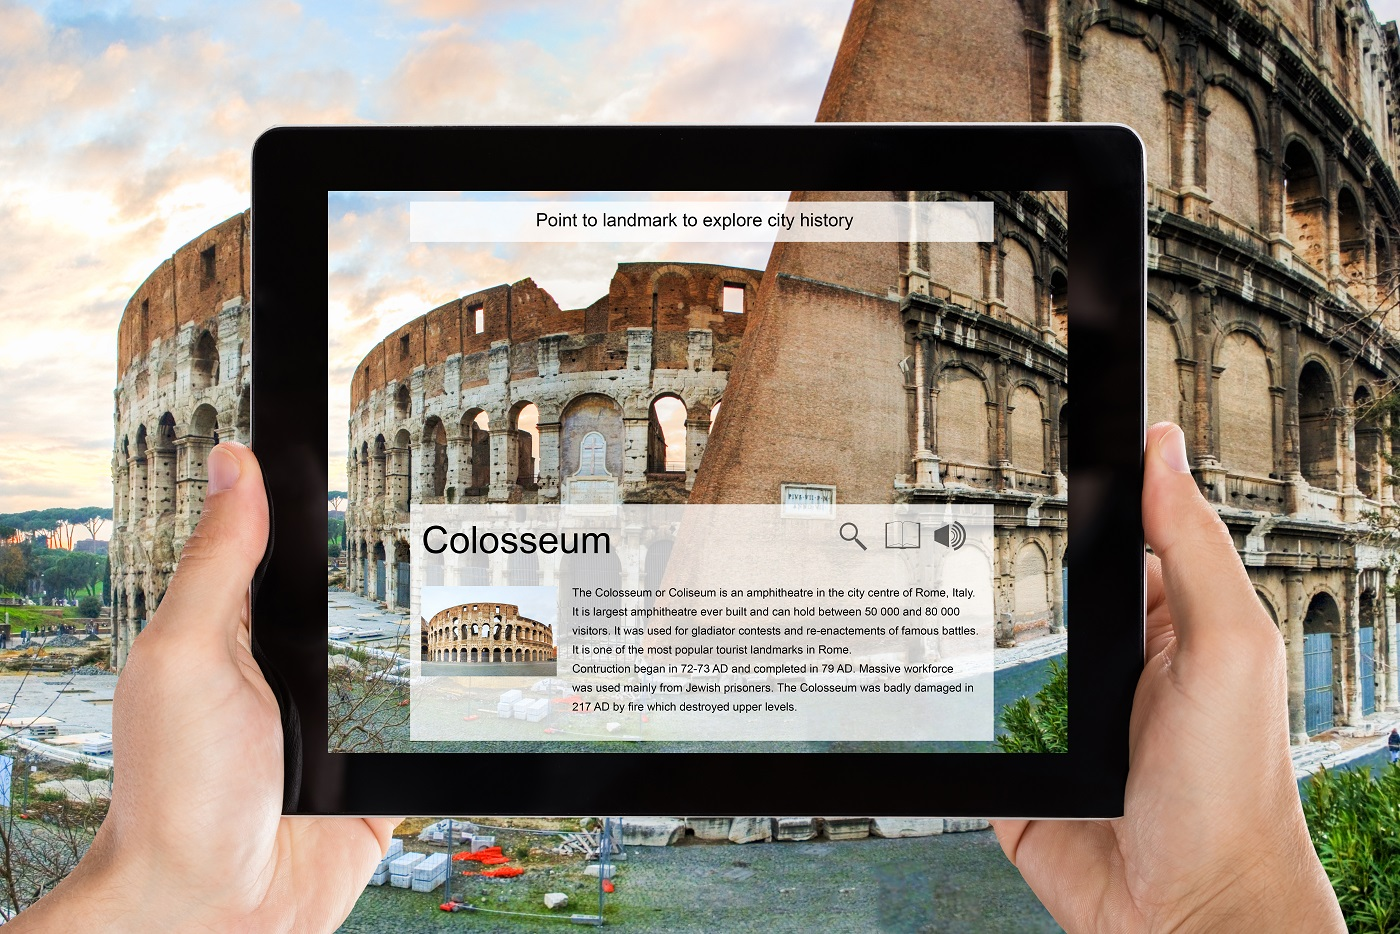
\includegraphics[width=0.8\textwidth]{ar.jpg}
\caption{АР технологија}
\end{figure}

\begin{figure}[H]
\centering
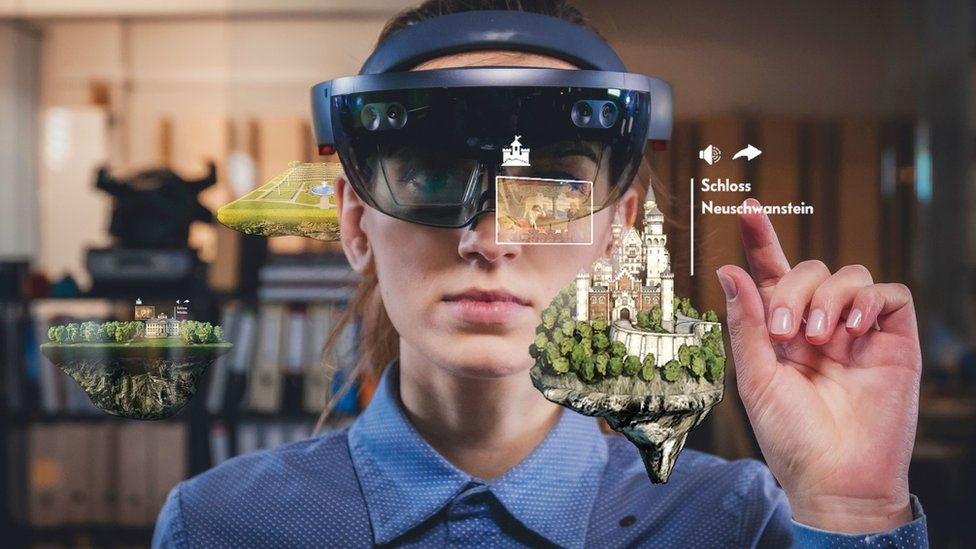
\includegraphics[width=0.8\textwidth]{vr.jpg}
\caption{ВР технологија}
\end{figure}

\section{Урбана разноликост и технологија}

Као што је речено у претходном одељку, индустрија путовања доживљава значајан раст захваљујући позитивним трансформацијама у транспортној индустрији, а све више кроз ваздушни саобраћај, који је повезао скоро све делове света, посебно велике градове. Овај раст је довео до повећања броја људи који путују на различите дестинације због посла, образовања, одмора и туризма. Такви трендови су довели до невиђене конкуренције у индустрији туризма и угоститељства, као и између градова који се позиционирају да привуку што већи број путника, посебно младих, за које се сматра да су авантуристички настројенији од свих других демографских група. Међу областима које добијају додатну пажњу је културни туризам, који интересује већину путника \cite{richardsg}. Стога путничке агенције и градови иновирају своје производе како би се уклопили у концепт културног туризма. Међутим, као што је горе наведено, кроз модерне идеологије планирања, већина оригиналног урбаног наслеђа бледи, пошто су зграде и други културни симболи рушени, уклоњени или подвргнути озбиљним реновирањем да би се ускладили са модернистичким перспективама. Такви трендови нису у складу са културним туризмом (као ни већина модернистичких идеологија планирања), што је довело до хомогено изграђених окружења, што ослабљује конкурентност, аутентичност и иновативност \cite{appendino}.

Упркос изазовима планирања, градови стварају иновативне начине, посебно коришћењем технологије за промовисање разноликости културе, што заузврат помаже у повећању њихове живахности и туристичких активности. Пример за то је Гугенхајмов музеј у Билбау, једно од најцењенијих дела савремене архитектуре \cite{archbilbao}, који је помогао у ревитализацији града и знатно повећао број домаћих и страних путника у жељи да посете музеј \cite{plazab}. Пројекат је био рађен према компјутерском програму и захваљујући томе су пројектвани такви облици који су били неизводљиви у традиционалним техникама градње. Недуго након отварања, Гугенхајм је постао популарна туристичка атракција, привлачећи посетиоце из целог света \cite{nytbilbao}. Још један недавни случај може се наћи у Петерсбургу у Кентакију, где Музеј уметности и стваралаштва капитализује моћ технологије и хришћанско веровање у стварање како би онима који посећују дао нову димензију и искуство теорије стварања \cite{hamk}.

\subsection{Апликације за промовисање садржаја који нуде градови}
Поред употребе технологије у архитектонском дизајну, технологије се такође широко користе за промоцију услуга, производа и различитих информација у вези са понудом културних производа у различитим градовима широм света. Са новим разорним технологијама мобилних уређаја, посебно кроз коришћење апликација, такмичење у промоцији градова као културних центара добија на замаху. Користе се за приказивање информација попут културних календара, културних локација и дељења слика уживо из различитих делова градова \cite{pietrol}. Такође, развијене су платформе за резервисање седишта, продају карата, вожњу таксијем по градовима и многе друге \cite{mckinsey}. Такве апликације раде на паметним телефонима и пажљиво су  брендиране коришћењем иновативних и најсавременијих технологија како би привукле што више корисника и потрошача. Пример такве апликације је \textit{Евентбрајт} који омогућава организаторима догађаја да путем апликације поставе релевантне информације о предстојећим догађајима и промовишу и продају виртуелне карте \cite{jamaluddina}. Апликација је прилагођена тако да корисници могу да претраже догађаје у свом локалитету или на било ком месту које можда планирају да посете. Још једна слична апликација је \textit{Филд Трип}, коју је направио и промовисао технолошки гигант \textit{Гугл} \cite{ingrahamn}. Ова апликација, уместо визуелног приказивања информација, повезује информације преко слушалица и садржи вредне информације о културним интересима као што су храна, историја, архитектура итд. Поред ових, једна вредна апликација коју градови користе за промоцију догађаја унутар свог периметра је \textit{Вамос}, моћна апликација која може да сними догађаје снимљене у другим апликацијама, па стога њени корисници не могу ништа пропустити у својим областима. Занимљиво је да је још један тренд који је произашао из све веће повезаности коју је донела технологија био \textit{co-working} (рад заједно), где радници различитих компанија деле пословни канцеларијски простор. Такве врсте простора се појављују у градовима широм света. Они су често подржани идентитетом који промовише разноликост и културно оријентисан бренд, за разлику од традиционалних распореда хладних канцеларија.

\begin{figure}[H]
\centering
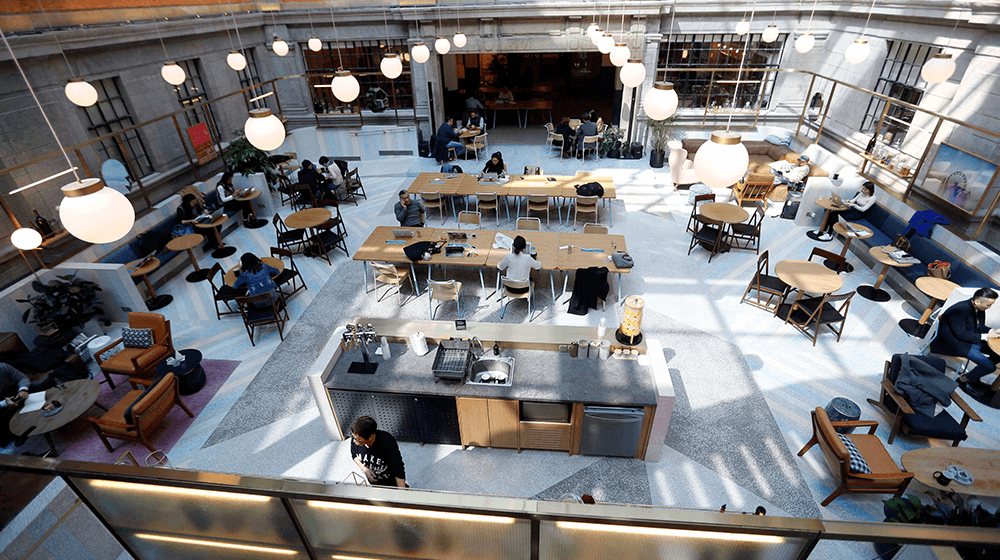
\includegraphics[width=0.76\textwidth]{co-work.png}
\caption{Co-working}
\end{figure}

\subsection{Брендирање градова}
Поред коришћења апликација, градови такође троше знатан износ својих буџета да се брендирају и ребрендирају користећи креативне идеје за промоцију осмишљавањем кратких слогана који би били карактеристични за тај град. Најпознатији од таквих брендова су: \textit{I Love New York}, \textit{IAMSTERDAM}, \textit{Nothing normal ever changed a damn thing} (Хелсинки), \textit{Let’s Make it Happen}  (Луксембург), \textit{State of COLORADO} и многи други \cite{theplace}. Такве идеје за брендирање намењене су да се интегришу у платформе друштвених медија под хештеговима који приказују кратке клипове, логотипе брендова, слике из градова и дискусије које се врте око тога шта такве градове чини супериорнијим у односу на друге и вредним посете. Сразмерно количини енергије и ресурса уложених у то, такве стратегије биле су веома успешне.

Овакво брендирање није фокусирано само на промоцију атрактивности града, већ се све више користи као алат за покретање концепта јединственог идентитета са којим би се могли повезати они који бораве или посећују град \cite{kavara}. Штавише, то се ради да би се промовисао концепт културне разноликости који је синоним за већину градова, који су временом постали „лонци за топљење” културе \cite{cotir}. Уз све ово, поставља се питање да ли ће свет у блиској будућности бити сведок нове урбане културе рођене укрштањем различитих група људи заједно са историјским наслеђем града \cite{burgess}. Када се то деси, такве културе ће поставити нове изазове градовима, а највероватнији је гажење постојећег културног наслеђа.

\begin{figure}[H]
\centering
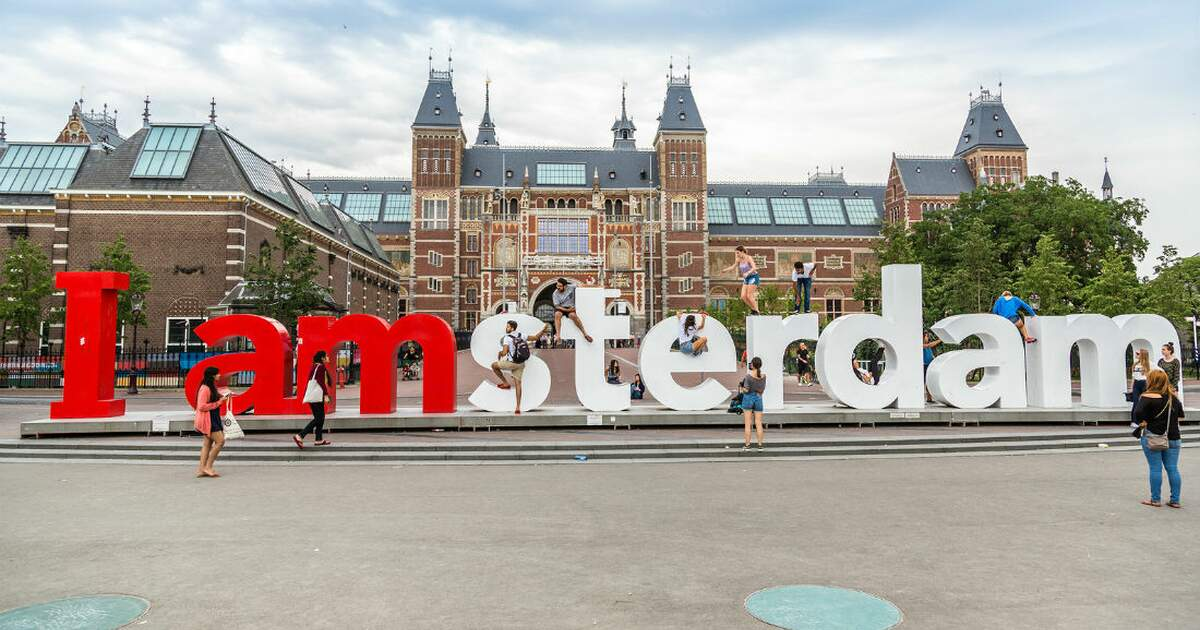
\includegraphics[width=0.9\textwidth]{amsterdam.jpg}
\caption{Логотип Амстердама}
\end{figure}

\begin{figure}[H]
\centering
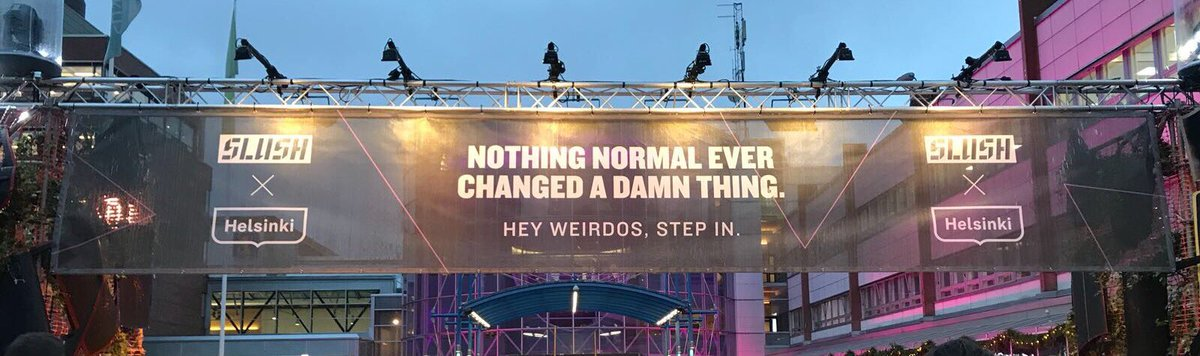
\includegraphics[width=0.9\textwidth]{helsinki.jpg}
\caption{Логотип Хелсинкија}
\end{figure}

\section{Аутономни градови и вештачка интелигенција}

Кључне улоге које градови играју у било којој економији су огромне и зато их треба заштитити по сваку цену. У овом контексту, градови журе да усвоје најбоље и најнапредније стратегије како би осигурали да остану у току са конкуренцијом и технологијама и да увек теже да савладају све веће урбане изазове. Срећом, због технолошког напретка, посебно у области управљања подацима, градови имају прилику да наставе да унапређују своје урбано ткиво. Већина података потиче са различитих платформи друштвених медија које посетиоци деле о граду и својим искуствима. Коришћење мобилних уређаја је постало свеприсутно у модерним данима, па стога постоји мноштво корисних података о скоро сваком аспекту урбаног ткива неког града. Сваки аспект града је подељен и присутан у друштвеним медијима, а ти подаци се могу користи за олакшавање и убрзање доношења неких одлука, што свеукупно може бити веома корисно у аспекту брендирања и побољшања културолошке разноликости \cite{alamjr}.

\subsection{Ефикаснија решења за јавне секторе}
Моћ вештачке интелигенције је веома велика и примењује се за доношење информисаних одлука о бројним питањима, јер најчешће то може да ради брже од људи. Вештачка интелигенција има потенцијал да доноси одлуке брже од било којих других процеса који су повезани са доношењем одлука. У вези с тим, вреди ценити предности које град може да извуче из аутономије. Прво, одлуке које се доносе би биле у реалном времену, непристрасне и засноване на великој количини података, па би стога имале далекосежне позитивне утицаје \cite{mohamed}. На пример, утицај аутономног саобраћајног сектора би спасио град од проблема као што су загушења и смањио ниво несрећа и грешака у вези са људима. Тако би се могла побољшати и ефикасност сектора попут здравства, енергетике и образовања, која би произашла из аутоматизације урбаних процеса \cite{norman}.

\subsection{Незаменљива улога човека}
Упркос чињеници да функције вештачке интелигенције пружају много користи, потенцијал да се у потпуности ослоне на њу, у одсуству било какве људске интервенције, некима још није изводљив. Ова технологија има потенцијал да превиди, занемари и понекад класификује неке секторе као мање важне за друге или насупрот питањима људског понашања \cite{dubey}. На пример, културни атрибути у једном граду могу бити класификовани као мање пожељни или битни у поређењу са осталима, а то су безбедност, здравство или образовање. У извесној мери, у кратком року, то може изгледати прихватљиво. Ипак, занемаривање културних аспеката града може имати лоше последице по економију града. Из тога се види да колико год је дигитализација урбаних центара донела бројне позитивне утицаје, улога човека је незаменљива \cite{zorins}. Процеси засновани на вештачкој интелигенцији не могу се поредити са људским способностима у доношењу одлука када се ради о спорним питањима. Стога, њима не могу управљати само технологије, а људи који доносе одлуке о суптилним стварима би требало увек да буду у првом плану \cite{heh}.

\section{Закључак}

Улога технологије у градовима мора бити пажљиво интегрисана како се не би подстакло прање јединствених културних тканина старих градова, јер мешање различитих култура, чак и ако се цени, мора бити пажљиво урађено. Коришћење технологије, кроз процесе вештачке интелигенције, у рачунарству аутономних градова мора се третирати са пажњом и сензибилношћу. Културни атрибути се не смеју негирати нити заједно груписати, јер као такви могу брзо да подстакну стварање хомогених простора. 

\newpage
\bibliographystyle{unsrt}
\bibliography{bibliography} 

\vspace{-7}
\bibitem{} [41] \space Allam, Z. Cities and the  Digital  Revolution Aligning technology and humanity. \emph{Digital Urban Networks and Social Media}, page 107-130, 2020.

\end{document}
